% !TeX root = ../../../main.tex
\subsubsection{Benchmarking on Real Data}
\label{ch04:sec:real-data}


We also evaluate the three families of survival CATE estimators on two real-world datasets, one with known ground truth and one without.





% !TeX root = ../../../main.tex
\begin{figure}[htbp]
\ChFourFloatContents{ch04:fig:twin30_rmse}{\caption{CATE RMSE for twin birth data with $h=30$ days across 10 experimental runs.}}{
  \centering
  
  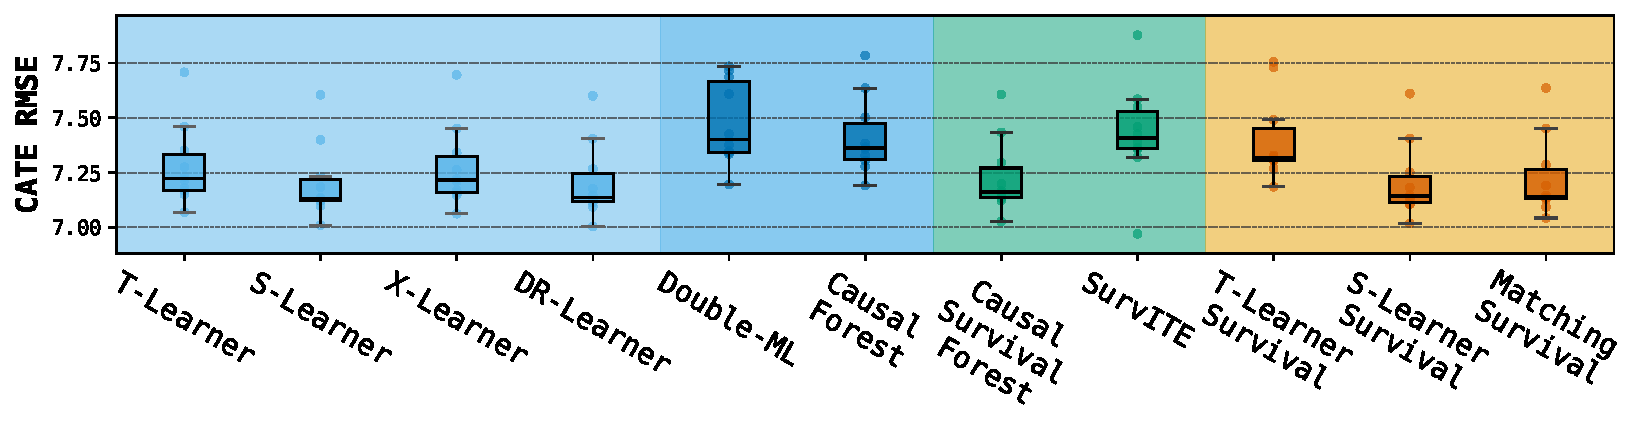
\includegraphics[width=1\linewidth]{Chapters/chapter-04/images/figure_results_updated/real_data/twin_scenario_1_twin30_cate_rmse.pdf}
  
   
}
\end{figure}



\textbf{Twin data.} The Twins dataset \citep{almond2005the,curth2021survite} includes twin births from 1989-1991, where being the heavier twin serves as treatment and time to mortality as the outcome. With known outcomes for both twins, this dataset provides ground truth for CATE evaluation. After replicating the same random treatment assignment strategy and the censoring time assignment following \cite{curth2021survite}, the treatment rate and censoring rate for the dataset are 68.1\% and 84.8\% respectively across 11,400 twin pairs. Since most of the mortality events occur within 30 days, we use $h=30$ days during estimation. 
Figure~\ref{ch04:fig:twin30_rmse} shows that S- and DR-Learners (with imputation) and S-Learner-Survival exhibit lower CATE RMSE (7.2 days).
T-Learner-Survival and Causal Forest with imputation exhibit the worst performance, consistent with their overall lower ranking from the benchmarking on our synthetic datasets (Figure~\ref{ch04:fig:average_rank_all}).
Surprisingly, Double-ML with imputation exhibits the worst performance on the twin data, which is different from the overall ranking, suggesting potential unique patterns in this dataset.
In Appendix~\ref{ch04:app:more-real-data-setup-result}, we also show the result with $h=180$ days; the conclusions are similar.



\textbf{HIV clinical trial.} The ACTG 175 dataset~\citep{hammer1996atrial} compared four antiretroviral treatments in 2,139 HIV-infected patients.
Following \cite{meir2025heterogeneous}, we convert time to months with $h$=30 months (13.7\% baseline censoring) and introduce artificial censoring to test robustness (increasing to $>$90\% censoring).
More details on data and processing can be found in Appendix~\ref {ch04:app:more-real-data-setup-result}. 
Figure~\ref{ch04:fig:hiv1-cate-estimate-comparison} compares CATE estimates between baseline and high-censoring conditions for the ZDV vs.~ZDV+ddI comparison (results for other treatment comparisons are in Appendix~\ref{ch04:app:more-real-data-setup-result}).
Each point represents an individual patient, with the 45-degree dashed line indicating perfect consistency between conditions.
We observe distinct behavioral patterns: Causal Survival Forest (green) produces estimates that cluster tightly around their original values; outcome imputation methods (blue) show higher variation in baseline estimates but concentrated predictions under high censoring; survival meta-learners (red) display substantial deviations from the 45-degree line, indicating sensitivity to censoring conditions.
As ground truth is unknown, we cannot determine which approach is more accurate, but these patterns reveal fundamental differences in how estimators respond to increased censoring.
For example, survival meta-learners (the red scatter plots), especially the T- and matching-learners, exhibit instability under increased censoring settings (large variance in y-axis values).


% !TeX root = ../../../main.tex
\begin{figure}[htbp]
\ChFourFloatContents{ch04:fig:hiv1-cate-estimate-comparison}{\caption{CATE estimation comparison between baseline and high-censoring conditions under ZDV vs. ZDV+ddI treatments. Each point represents an individual patient, with the dashed diagonal line indicating perfect consistency between baseline CATE estimation and that with the additional censoring injected.}}{
  \centering
  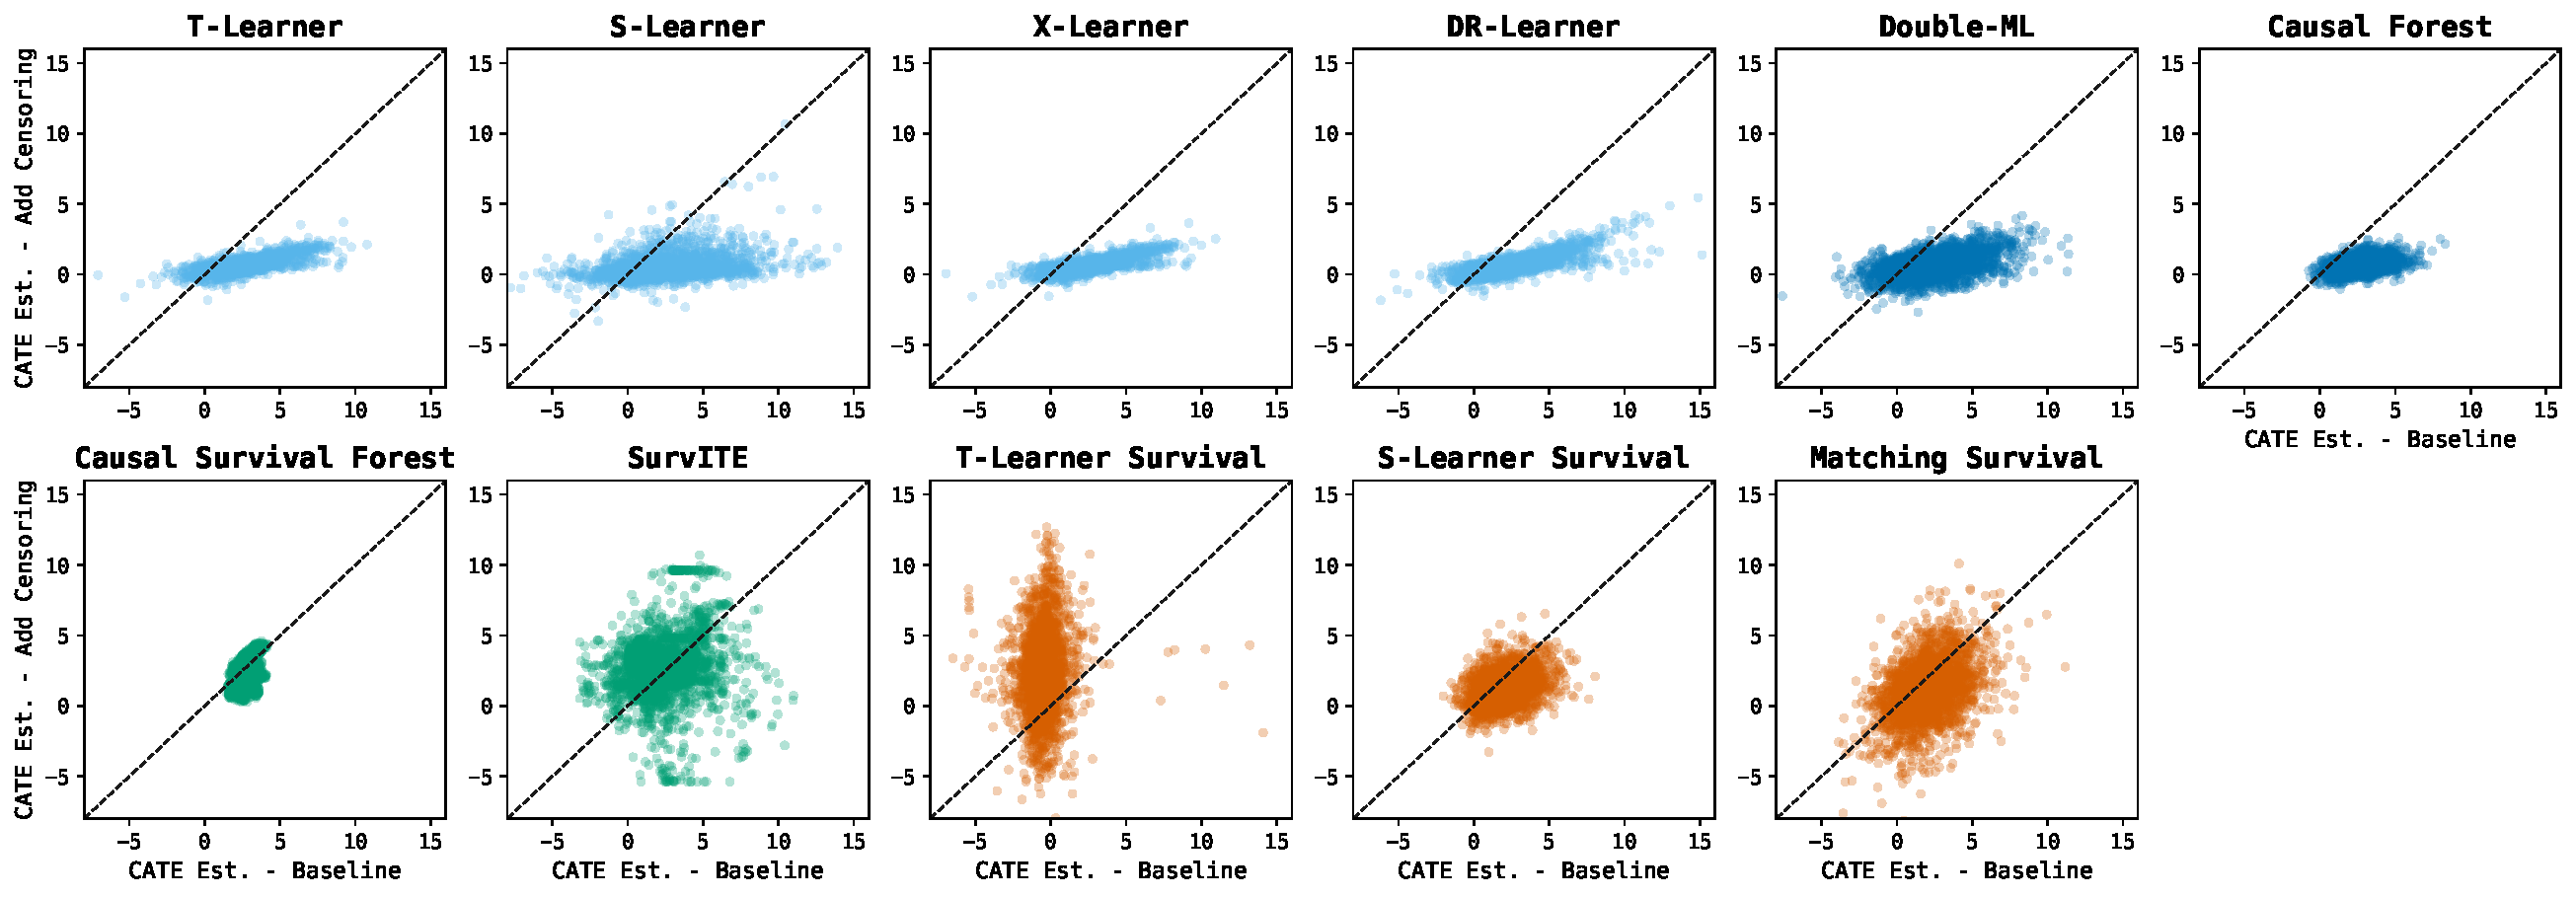
\includegraphics[width=0.95\linewidth]{Chapters/chapter-04/images/figure_results_updated/real_data/ACTG_175_HIV1_CATE_comparison.pdf}
   
}
\end{figure}



